%!TEX root = ../../thesis.tex

A statistical model is built within the \histfactory software package \cite{HistFactory}, 
incorporating the various data-driven techniques described in Chapters~\ref{chap:ww} and 
\ref{chap:backgrounds}. The experimental data and MC-modelled expectations found within each 
signal and control region allow the model to be constrained, and for various hypotheses to 
be tested.



\subsection{Discriminant observables}
\label{sec:stat:sr_binning}

The fitting procedure discriminates between the signal and background processes through the 
distribution of certain sensitive observables. However, the degree to which this information 
can be exploited is limited by statistical uncertainties. The sensitivity of the fitting 
procedure can be optimised through the choice of discriminating observables, the number of 
bins in each observable, and the location of the bin boundaries.

The analysis features eight signal regions, defined by the criteria in 
\Section~\ref{sec:selection}: $\braces{\emch,\mech,\eech{}+\mmch} \otimes 
\braces{\text{0-jet,1-jet}}~~\oplus~~\braces{\emch,\mech} \otimes \braces{\twojet}$.
A three-dimensional fit of \mt, \ptsubleadlep and \mll is performed in the 
$\braces{\emch,\mech} \otimes \braces{\text{0-jet,1-jet}}$ signal regions, whereas a 
one-dimensional \mt fit is used in the others.

Additionally, in the $\braces{\emch,\mech,\eech{}+\mmch} \otimes \braces{\text{0-jet,1-jet}}$
signal regions, the \mt bin boundaries are chosen such that there are an equal number of 
expected signal events in each bin. This is applied independently within each 
\ptsubleadlep-\mll bin in the \emch/\mech channels. In the \twojet bin, fixed \mt bin 
boundaries are used.

The binning of each discriminant observable is shown in \Table~\ref{tab:stat:sr_binning}, 
and the inclusive \mt distribution of each jet bin is shown in \Figure~\ref{fig:results:mt}.

\begin{table}[t]
	\begin{tabular}{cc@{\hskip 0.3in}ccc@{\hskip 0.3in}c}
		\toprule
		\multirow{2}{*}{\njets} & \multirow{2}{*}{Channel} & \multicolumn{3}{c}{Bin boundaries (\GeV)} & \multirow{2}{*}{$N_{\text{bins}}$} \\
		& & \ptsubleadlep & \mll & \mt & \\
		\midrule
		0-jet & \emch, \mech   & \hardrange{10,15,20,\infty} & \hardrange{10,30,55} & 10 bins & 60 \\
		0-jet & \eech{}+\mmch  & \hardrange{10,\infty} & \hardrange{12,55} & 10 bins & 10 \\
		1-jet & \emch, \mech   & \hardrange{10,15,20,\infty} & \hardrange{10,30,55} & \phantom{1}6 bins & 36 \\
		1-jet & \eech{}+\mmch  & \hardrange{10,\infty} & \hardrange{12,55} & \phantom{1}6 bins & 6 \\
		\twojet & \emch, \mech & \hardrange{10,\infty} & \hardrange{10,55} & \hardrange{0,50,80,130,\infty} & 4 \\
		\bottomrule
	\end{tabular}
	\caption{The binning of each discriminant observable for each signal region. The \mt 
	bin boundaries in the 0-jet and 1-jet bins are chosen to produce a flat signal.}
	\label{tab:stat:sr_binning}
\end{table}

\begin{figure}[p]
	\null\hfill
	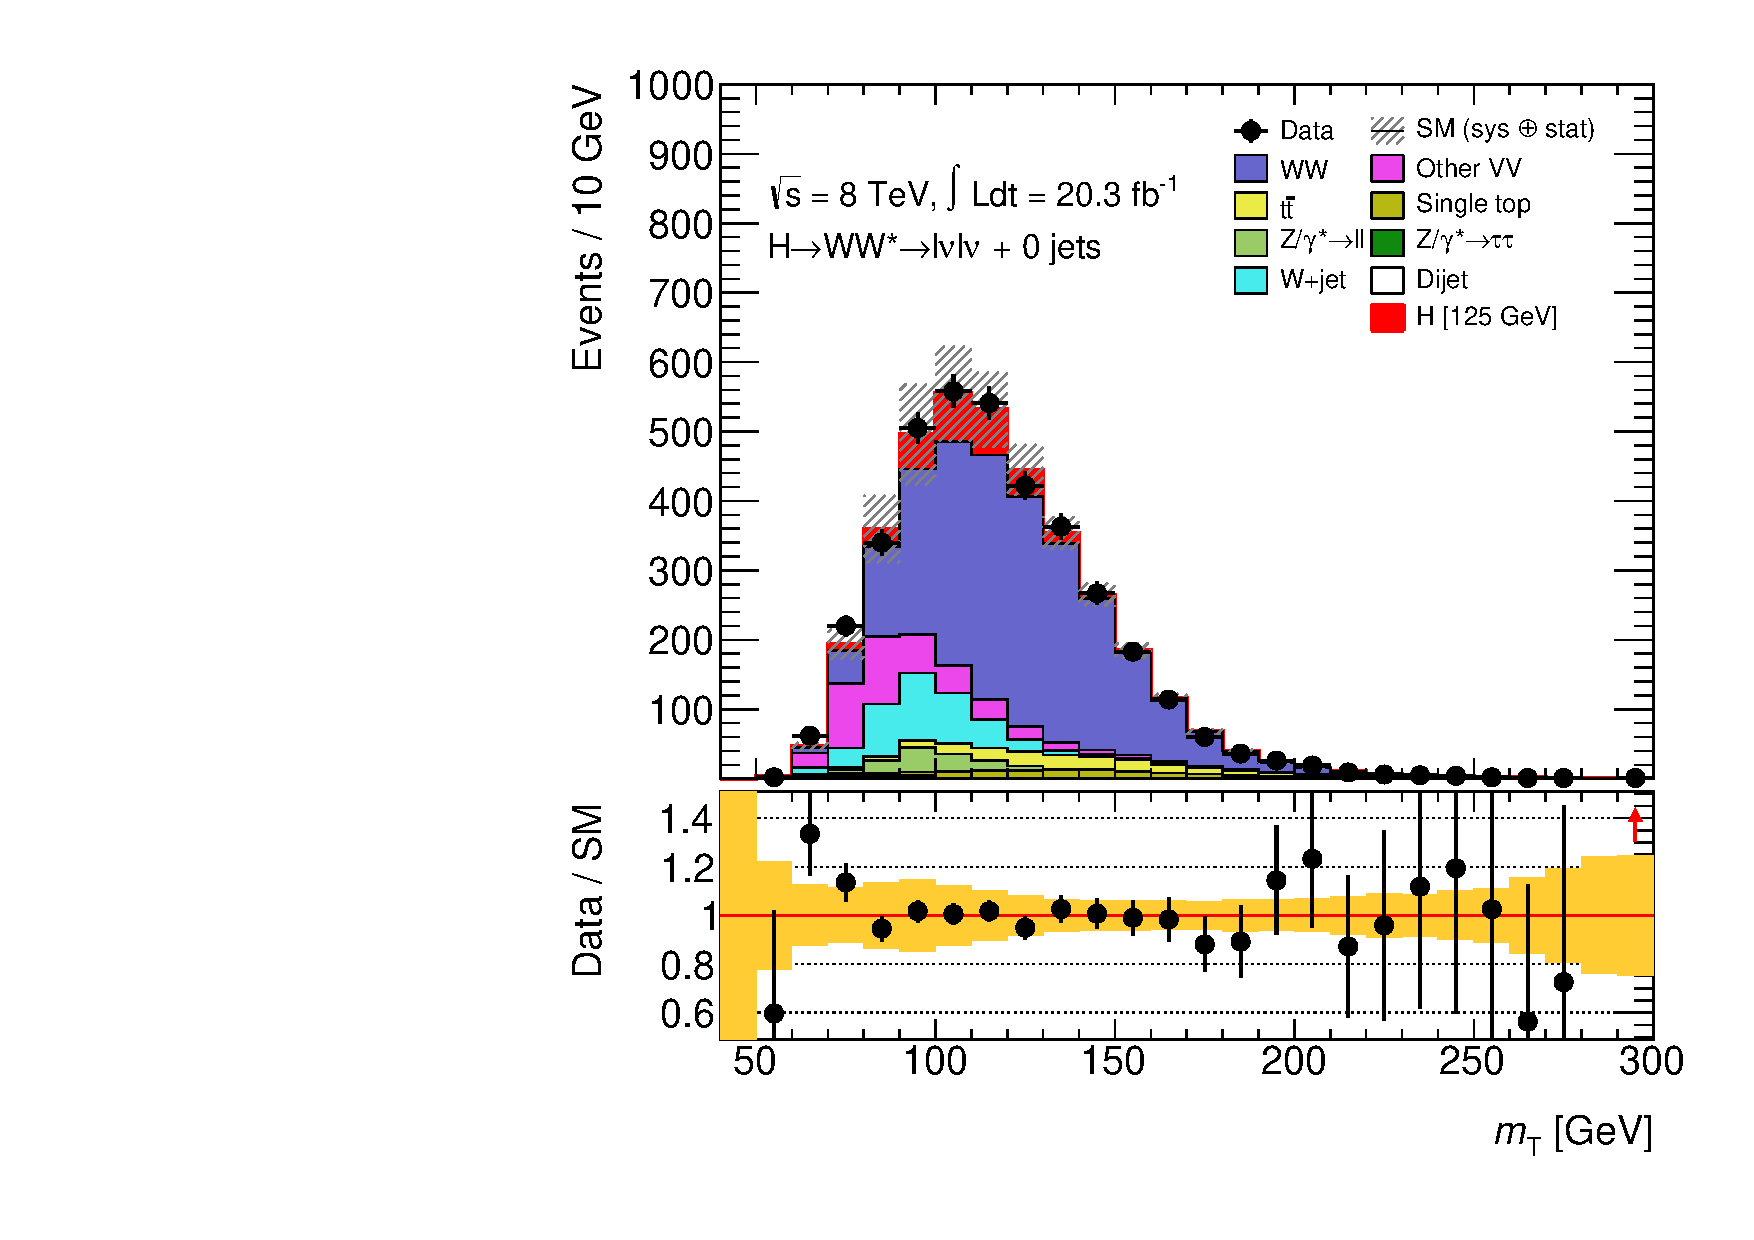
\includegraphics[width=0.49\textwidth]{tex/results/CutFRecoil_0jet_MT_TrackHWW_Clj_mh125_lin}
	\hfill
	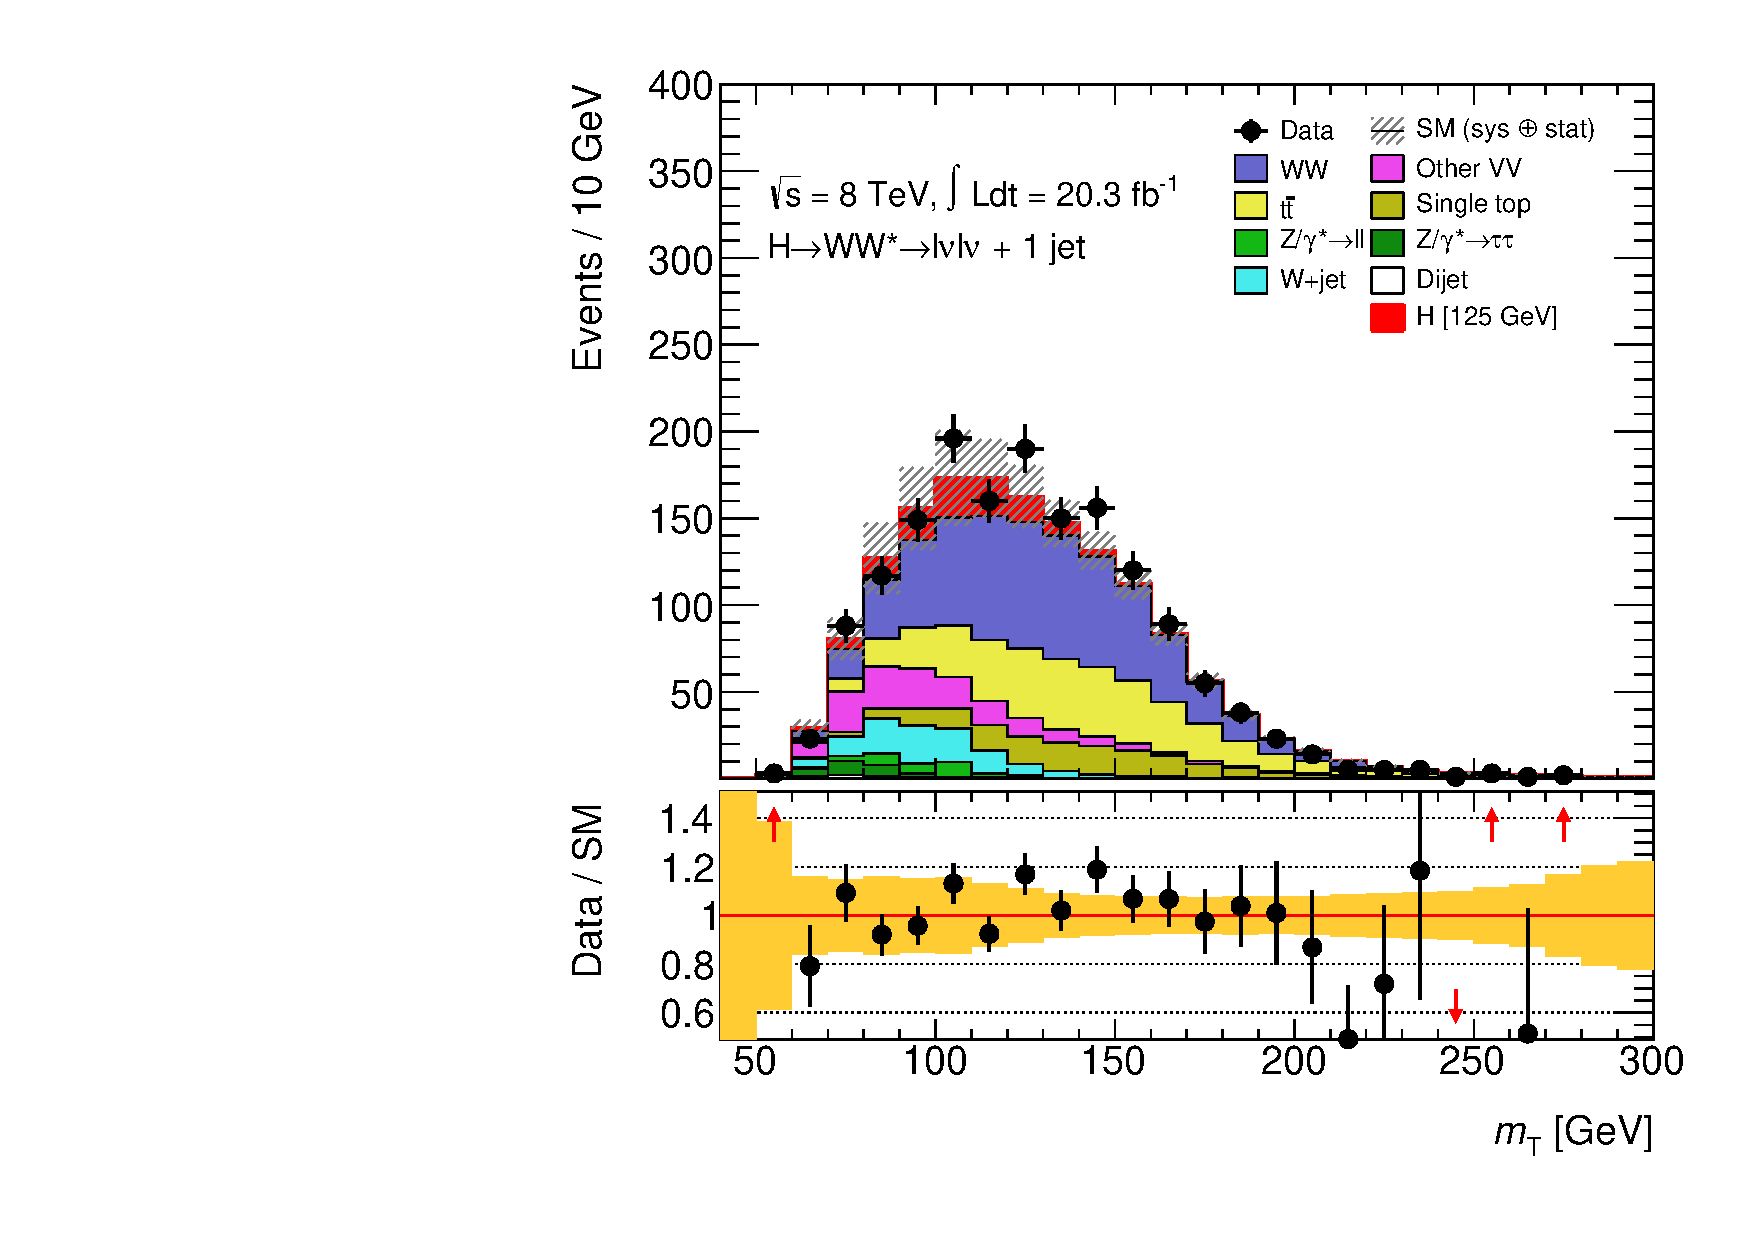
\includegraphics[width=0.49\textwidth]{tex/results/CutFRecoil_1jet_MT_TrackHWW_Clj_mh125_lin}
	\hfill\null
	\\
	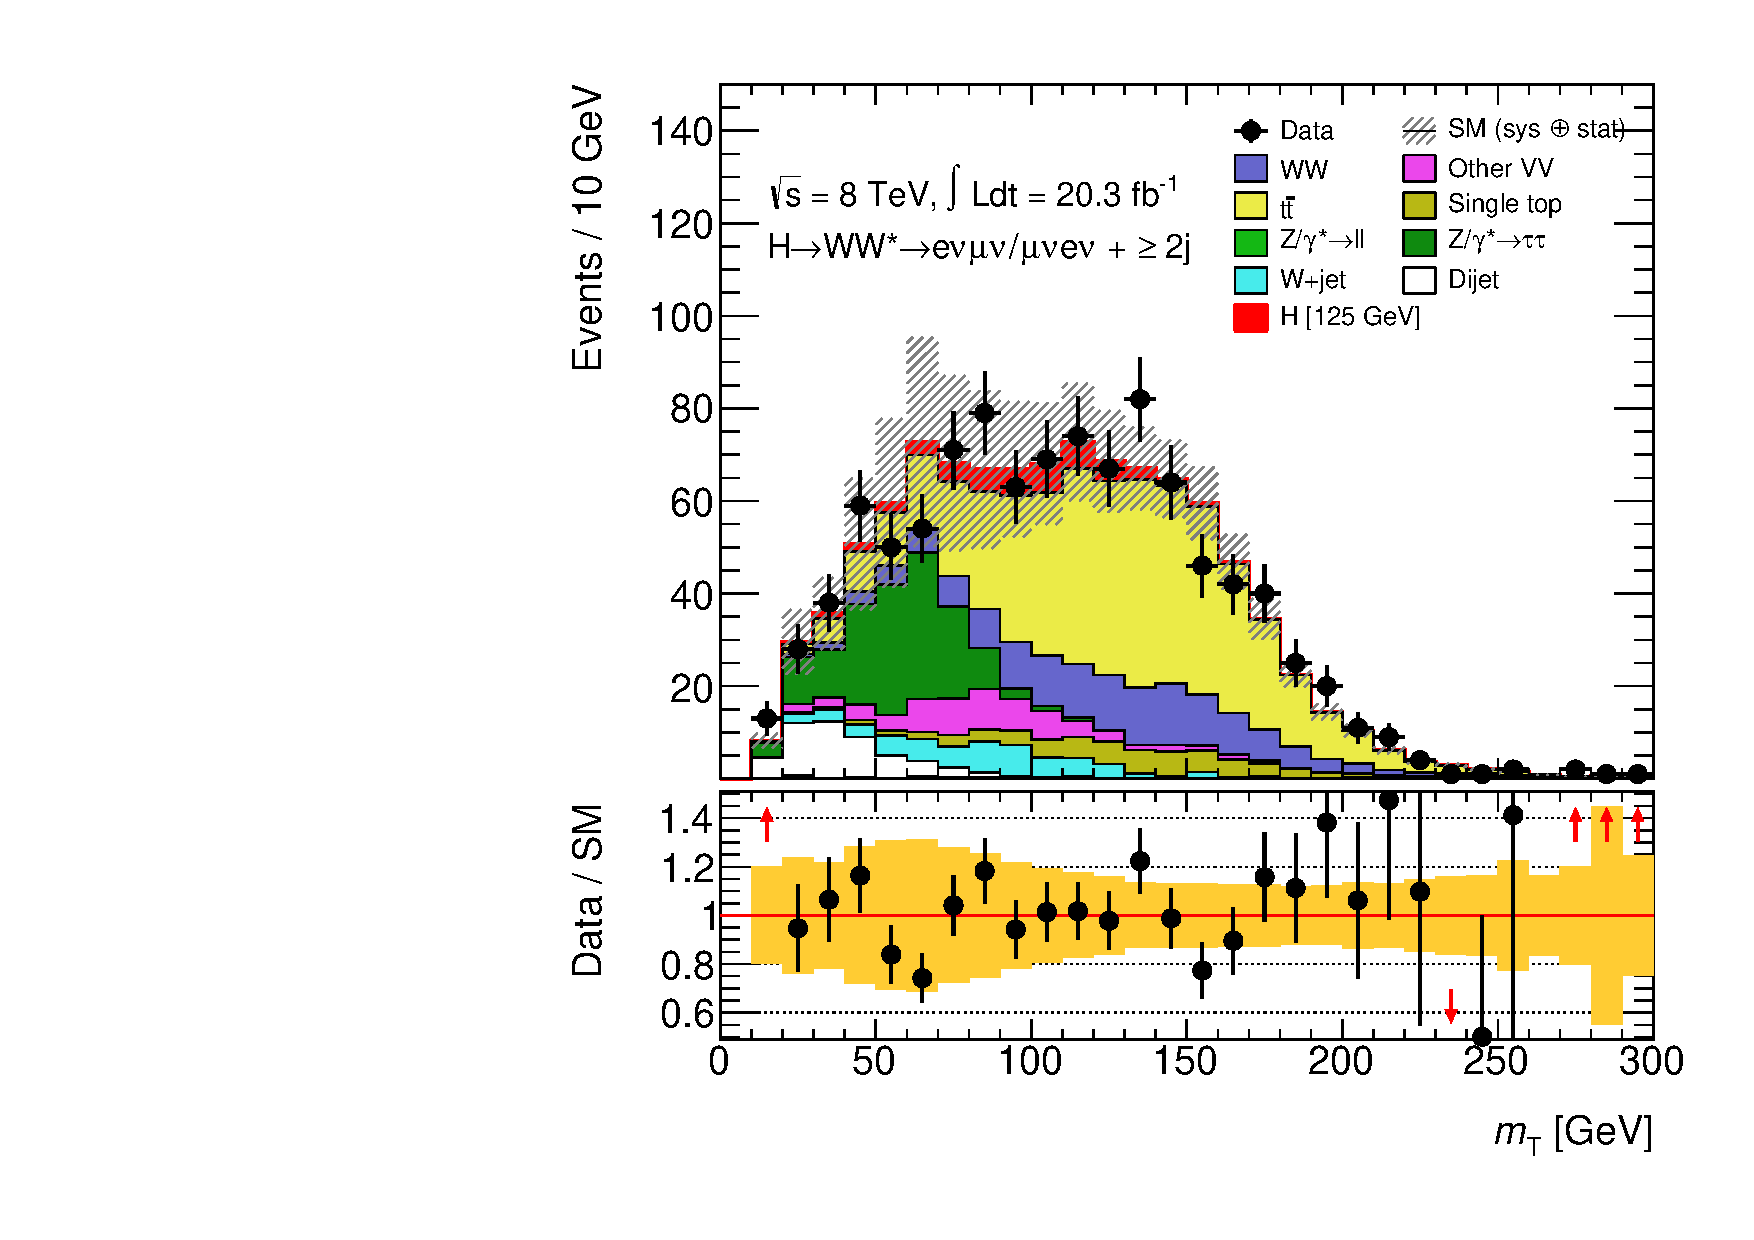
\includegraphics[width=0.49\textwidth]{tex/selection/\blindfolder/emme_CutFailVBFTopoDPhillggFlike_2jetincl_MT_TrackHWW_Clj_mh125_lin}
	\caption{The \mt distribution in the signal region of the 0-jet (left), 1-jet 
	(right) and \twojet (bottom) bin. Normalisation factors are applied.}
	\label{fig:results:mt}
\end{figure}



\newpage
\subsection{Likelihood function}
\label{sec:stat:likelihood}

The statistical model describing the experiment depends upon a set of parameters 
$\bvec{\alpha} = \parenths{\mu, \bvec{\theta}}$, where $\mu = \sigma/\sigma_{\text{SM}}$ is 
the signal strength (a parameter of interest) and \bvec{\theta} is the set of nuisance 
parameters (\eg trigger efficiency, \WW extrapolation parameter $\alpha_{\WW}$). The Higgs 
boson mass \mH could also be treated as a parameter of interest, but hypothesis testing is 
usually performed as a raster scan of \mH in practice.

The likelihood function expresses how likely a set of parameter values are, given that a 
particular dataset is observed. It is defined as the probability of producing the observed 
dataset, when the parameter values are input into the statistical model,
\begin{equation}
	\mathcal{L}\parenths{\mu, \bvec{\theta}} &= \mathcal{L}\parenths{\mu, \bvec{\theta} ~\given~ \bvec{\mathcal{D}^{\text{SR}}}, \bvec{\mathcal{D}^{\text{CR}}}} \\
	&= f\parenths{\bvec{\mathcal{D}^{\text{SR}}}, \bvec{\mathcal{D}^{\text{CR}}}; \,\mu, \bvec{\theta}}
\end{equation}
where \bvec{\mathcal{D}^{\text{SR}}} and \bvec{\mathcal{D}^{\text{CR}}} are the 
observed datasets in the signal regions (SRs) and control regions (CRs), respectively.
This can be decomposed into a product of probabilities
\begin{equation}
	\mathcal{L}\parenths{\mu, \bvec{\theta}} = \!\!\!\!\!\prod\limits_{c\in\text{channels}} \!\!\!\!\!f\parenths{\mathcal{D}_{c}^{\text{SR}}; \,\mu, \bvec{\theta}} ~\!\!\!\!\!\prod\limits_{c\in\text{channels}}\!\!\!\!\! f\parenths{\mathcal{D}_{c}^{\text{CR}}; \,\mu, \bvec{\theta}} \prod\limits_{i\in\text{n.p.}} f_i(\tilde{\theta}_i; \,\theta_i, \Delta\tilde{\theta}_i)
\end{equation}
where the SR channels are the eight SRs described in \Section~\ref{sec:stat:sr_binning}, and 
the CR channels include the data used in data-driven background estimations. Each 
$f_i(\tilde{\theta}_i; \,\theta_i, \Delta\tilde{\theta}_i)$ acts to constrain the 
corresponding nuisance parameter, and is often a Gaussian distribution. The nominal value 
$\tilde{\theta}$ and uncertainty $\Delta\tilde{\theta}$ are determined by an auxiliary 
measurement, either experimental (\eg trigger efficiency) or theoretical (\eg 
$\alpha_{\WW}$).

The probability of producing an observed distribution $\mathcal{D}_c$ is described by 
a product of Poisson distributions
\begin{equation}
	f\parenths{\mathcal{D}_c; \,\mu, \bvec{\theta}} &= \!\prod\limits_{b\in\text{bins}}\! \Pois{N_{cb}^{\text{obs}}; \,\mu N_{cb}^{\text{sig}}\parenths{\bvec{\theta}} + N_{cb}^{\text{bkg}}\parenths{\bvec{\theta}}}
\end{equation}
where $\Pois{x; \,\lambda} = \lambda^x \eexp{-\lambda} / x!$, $N_{cb}^{\text{obs}}$ is the 
number of observed events, $N_{cb}^{\text{sig}}\parenths{\bvec{\theta}}$ is the number of 
expected signal events for a Standard Model Higgs boson (estimated by MC), and 
$N_{cb}^{\text{bkg}}\parenths{\bvec{\theta}}$ is the number of expected background events 
(estimated by data-driven techniques embedded in the statistical model). The product is over 
the bins of the distribution $\mathcal{D}_c$, which is one- or three-dimensional in the case 
of the SRs, and zero-dimensional in many of the CRs (\ie a single bin).

The expected numbers of events depend upon the nuisance parameters according to
\begin{equation}
	N_{cb}^{\text{sig}}\parenths{\bvec{\theta}} &= N_{cb}^{\text{sig}}(\tilde{\bvec{\theta}}) \prod\limits_{i\in\text{n.p.}} \nu_{cbi}(\theta_i - \tilde{\theta}_i) \\
	N_{cb}^{\text{bkg}}\parenths{\bvec{\theta}} &= \!\!\!\!\!\sum\limits_{p\in\text{processes}}\!\!\!\!\! N_{cbp}^{\text{bkg}}(\tilde{\bvec{\theta}}) \prod\limits_{i\in\text{n.p.}} \nu_{cbpi}(\theta_i - \tilde{\theta}_i)
\end{equation}
where $N(\tilde{\bvec{\theta}})$ is the expected events with the nominal nuisance parameters 
as determined by auxiliary measurements, and $\nu_i(\theta_i - \tilde{\theta}_i)$ factorises 
the dependence upon the nuisance parameter $\theta_i$. The 
$\nu_i(\theta_i - \tilde{\theta}_i)$ are often determined by evaluating 
$\nu_i(+\Delta\tilde{\theta}_i)$ and $\nu_i(-\Delta\tilde{\theta}_i)$, and then 
interpolating and extrapolating. Some nuisance parameters affect all processes (\eg trigger 
efficiency), whilst others only affect a particular process (\eg $\alpha_{\WW}$). 
Correlations can exist between bins and channels, \eg the 
$\nu_i(\theta_i - \tilde{\theta}_i)$ for a normalisation parameter would be 100\% 
correlated between bins. Statistical uncertainties in the MC samples are implemented as 
uncorrelated uncertainties in the total expected events in each bin, where the corresponding 
constraint $f_i(\tilde{\theta}_i; \theta_i, \Delta\tilde{\theta}_i)$ is a Poisson 
distribution.



\subsection{Hypothesis testing}
\label{sec:stat:tests}

The statistical techniques of hypothesis testing employed by Higgs boson searches at the LHC 
are fully described in references~\cite{Cowan:2010,Cranmer:lectures}. Those used in the \HWW 
search to exclude, discover and measure the Higgs boson are briefly summarised below.

Hypothesis testing is based around the profile likelihood ratio, defined as
\begin{equation}
	\lambda\parenths{\mu} = \frac{\mathcal{L}(\mu, \hat{\hat{\bvec{\theta}}}\parenths{\mu})}{\mathcal{L}(\hat{\mu}, \hat{\bvec{\theta}})}
\end{equation}
where $\hat{\mu}$ and $\hat{\bvec{\theta}}$ are the parameter values that maximise the 
likelihood, and $\hat{\hat{\bvec{\theta}}}\parenths{\mu}$ are the nuisance parameter values 
that maximise the likelihood when $\mu$ is fixed. Maximal agreement with experimental data 
is expressed by the maximum $\lambda\parenths{\hat{\mu}} = 1$, and statistical and 
systematic uncertainties determine the shape of $\lambda\parenths{\mu}$. The maximised 
$\hat{\bvec{\theta}}$ and $\hat{\hat{\bvec{\theta}}}\parenths{\mu}$ can be pulled, and 
constrained differently, with respect to the auxiliary measurements $\tilde{\bvec{\theta}}$. 
An alternative version of the profile likelihood ratio is defined as
\begin{equation}
	\tilde{\lambda}\parenths{\mu} = 
	\begin{dcases*}
		\frac{\mathcal{L}(\mu, \hat{\hat{\bvec{\theta}}}\parenths{\mu})}{\mathcal{L}(\hat{\mu}, \hat{\bvec{\theta}})} & if $\hat{\mu} \geq 0$ \\
		\frac{\mathcal{L}(\mu, \hat{\hat{\bvec{\theta}}}\parenths{\mu})}{\mathcal{L}(0, \hat{\hat{\bvec{\theta}}}\parenths{0})} & if $\hat{\mu} < 0$
	\end{dcases*}
\end{equation}
which limits the model to $\hat{\mu} \geq 0$.

Frequentist techniques are used to test three different scenarios. First, we attempt to 
exclude a Standard Model (\ie $\mu = 1$) Higgs boson at the 95\% confidence level (CL), by 
testing $\mu < 1$. Second, we attempt to discover a Higgs boson (\ie $\mu \neq 0$) with 
$\geq\!5\sigma$ significance, by testing $\mu > 0$. Third, we make a measurement of the 
signal strength $\mu$ (with a two-sided confidence interval). Each scenario is tested as 
a raster scan of \mH.

Under each scenario (detailed below), a test statistic is constructed to quantify the 
disagreement between the observed data and a null hypothesis. A $p$-value is then 
computed, which is the probability of observing a test statistic at least as extreme as that 
observed, under the assumption of the null hypothesis. The $p$-value is computed by 
integrating a sampling distribution of the test statistic, which is based upon the 
likelihood function. This is done using an asymptotic formula, which is valid in the 
large-sample limit, though an ensemble of pseudoexperiments could be used instead 
\cite{Cowan:2010}. The validity of the asymptotic formula for this analysis has previously 
been checked against pseudoexperiments.

Finally, the median confidence levels expected under the assumption of an alternative 
hypothesis are calculated. This is done using a single pseudoexperiment, known as the Asimov 
dataset, corresponding to the \textit{exact} expectation (\ie pseudodata with fractional 
numbers of events) \cite{Cowan:2010}.

\begin{description}
\item[Exclusion] \hfill \\
	To determine an upper limit on the signal strength, a one-sided test statistic is 
	constructed under the assumption of a signal-plus-background null hypothesis:
	\begin{equation}
		\tilde{q}_{\mu} = 
		\begin{dcases*}
			-2 \ln \tilde{\lambda}\parenths{\mu} & if $\hat{\mu} \leq \mu$ \\
			0 & if $\hat{\mu} > \mu$
		\end{dcases*}
	\end{equation}
	where use of $\tilde{\lambda}\parenths{\mu}$ ensures that only $\mu \geq 0$ is 
	considered physical. The compatibility of the data with the null hypothesis is 
	quantified by the $p$-value
	\begin{equation}
		p_{\mu} = \int\limits_{\tilde{q}_{\mu,\text{obs}}}^{\infty} \! f(\tilde{q}_{\mu}~\given~\mu, \hat{\hat{\bvec{\theta}}}(\mu)) \,\, \d{\tilde{q}_{\mu}}
	\end{equation}
	where $f(\tilde{q}_{\mu}~\given~\mu, \hat{\hat{\bvec{\theta}}}(\mu))$ is the sampling 
	distribution of the test statistic under the assumption of an underlying signal strength 
	$\mu$, and $\tilde{q}_{\mu,\text{obs}}$ is the observed test statistic under the same 
	assumption. Thus, a 95\% CL upper limit upon $\mu$ is set at the value which satisfies 
	$p_{\mu} = 0.05$.

	An unfortunate feature of this method is that a downward fluctuation in the observed 
	data can exclude models where little sensitivity is expected. For this reason the 
	modified frequentist \CLs technique is used \cite{Junk:CLs,Read:CLs}, which defines the 
	$p$-value
	\begin{equation}
		p_{\mu}' = \frac{p_{\mu}}{1 - p_{b}}
	\end{equation}
	where incompatibilities with the null hypothesis are down-weighted if the data is also 
	incompatible with the background-only hypothesis, through
	\begin{equation}
		p_{b} = \int\limits_{-\infty}^{\tilde{q}_{\mu,\text{obs}}} \! f(\tilde{q}_{\mu}~\given~0, \hat{\hat{\bvec{\theta}}}(0)) \,\, \d{\tilde{q}_{\mu}} \,.
	\end{equation}
	Thus, a 95\% CL upper limit upon $\mu$ is set at the value which satisfies 
	$p_{\mu}' = 0.05$. The Standard Model Higgs boson is considered excluded if $\mu < 1$ at 
	the 95\% CL. The exclusion sensitivity is evaluated by calculating the expected $\mu$ 
	upper limit under the assumption of a background-only alternative hypothesis.

\item[Discovery] \hfill \\
	For discovery, a one-sided test statistic is constructed under the assumption of a 
	background-only null hypothesis:
	\begin{equation}
		q_0 = 
		\begin{dcases*}
			-2 \ln \lambda\parenths{0} & if $\hat{\mu} \geq 0$ \\
			0 & if $\hat{\mu} < 0$ \,.
		\end{dcases*}
	\end{equation}
	The compatibility of the data with the null hypothesis is quantified by the $p$-value
	\begin{equation}
		p_{0} = \int\limits_{q_{0,\text{obs}}}^{\infty} \! f(q_{0}~\given~0, \hat{\hat{\bvec{\theta}}}(0)) \,\, \d{q_{0}} \,.
	\end{equation}
	The Higgs boson is considered discovered if the background-only hypothesis is excluded 
	with $p_0 < 2.87 \times 10^{-7}$, corresponding to a significance of at least five 
	standard deviations (\ie $\geq\!5\sigma$) in a Gaussian distribution. The discovery 
	sensitivity is evaluated by calculating the expected $p_0$ under the assumption of a 
	signal-plus-background alternative hypothesis, with $\mu = 1$. As seen in 
	\Section~\ref{sec:results}, an \mH value must also be chosen for this hypothesis.

\item[Measurement] \hfill \\
	For the $\mu$ measurement, a two-sided test statistic is constructed under the 
	assumption of a signal-plus-background null hypothesis:
	\begin{equation}
		t_{\mu} = -2 \ln \lambda\parenths{\mu} \,.
	\end{equation}
	The compatibility of the data with the null hypothesis is quantified by the $p$-value
	\begin{equation}
		p_{\mu} = \int\limits_{t_{\mu,\text{obs}}}^{\infty} \! f(t_{\mu}~\given~\mu, \hat{\hat{\bvec{\theta}}}(\mu)) \,\, \d{t_{\mu}} \,.
	\end{equation}
	The nominal $\mu$ value will be $\hat{\mu}$, and the 68\% CL confidence interval is 
	set by the values which	satisfy $p_{\mu} = 0.16$. The measurement sensitivity is 
	evaluated by calculating the expected $\Delta\mu$ under the assumption of a 
	signal-plus-background hypothesis, with $\mu = 1$. Again, an \mH value must be chosen 
	for this hypothesis.

\end{description}


